\documentclass[border=2mm]{standalone}
\usepackage{tikz}
\begin{document}

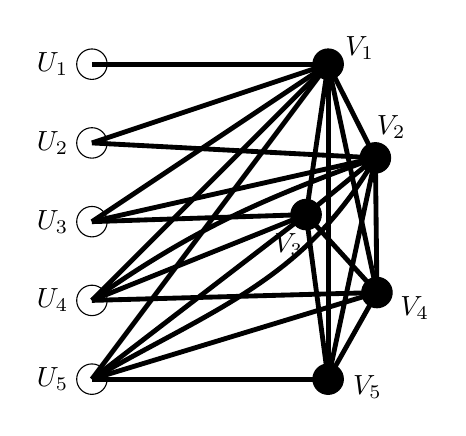
\begin{tikzpicture}
  % Define and draw left-side nodes U1 to U5 (unfilled circles with labels)
  \foreach \y/\name in {-3/U_1, -4/U_2, -5/U_3, -6/U_4, -7/U_5} {
    \draw (-7,\y) circle (5.5pt);
    \node at (-7.5,\y) {$\name$};
  }

  % Define and draw right-side nodes V1 to V5 (filled circles with labels)
  \draw [fill=black] (-4,-3) circle (5.5pt);
  \node[color=black] at (-3.6,-2.8) {$V_1$};

  \draw [fill=black] (-3.4,-4.19) circle (5.5pt);
  \node[color=black] at (-3.2,-3.8) {$V_2$};

  \draw [fill=black] (-4.28,-4.91) circle (5.5pt);
  \node[color=black] at (-4.5,-5.3) {$V_3$};

  \draw [fill=black] (-3.38,-5.9) circle (5.5pt);
  \node[color=black] at (-2.9,-6.1) {$V_4$};

  \draw [fill=black] (-4,-7) circle (5.5pt);
  \node[color=black] at (-3.5,-7.1) {$V_5$};

  % Draw vertical backbone edge on the right
  \draw [line width=1.75pt] (-4,-3) -- (-4,-7);

  % Draw internal edges among V-nodes
  \draw [line width=1.75pt] (-4,-3) -- (-3.4,-4.19);
  \draw [line width=1.75pt] (-3.4,-4.19) -- (-3.38,-5.9);
  \draw [line width=1.75pt] (-3.38,-5.9) -- (-4,-7);
  \draw [line width=1.75pt] (-3.4,-4.19) -- (-4,-7);
  \draw [line width=1.75pt] (-4,-3) -- (-4.28,-4.91);
  \draw [line width=1.75pt] (-4,-3) -- (-3.38,-5.9);
  \draw [line width=1.75pt] (-4.28,-4.91) -- (-4,-7);
  \draw [line width=1.75pt] (-4.28,-4.91) -- (-3.4,-4.19);
  \draw [line width=1.75pt] (-4.28,-4.91) -- (-3.38,-5.9);

  % Draw edges from each U-node to various V-nodes
  % From U1 = (-7,-3)
  \draw [line width=1.75pt] (-7,-3) -- (-4,-3);

  % From U2 = (-7,-4)
  \draw [line width=1.75pt] (-7,-4) -- (-4,-3);
  \draw [line width=1.75pt] (-7,-4) -- (-3.4,-4.19);

  % From U3 = (-7,-5)
  \draw [line width=1.75pt] (-7,-5) -- (-4,-3);
  \draw [line width=1.75pt] (-7,-5) -- (-3.4,-4.19);
  \draw [line width=1.75pt] (-7,-5) -- (-4.28,-4.91);

  % From U4 = (-7,-6)
  \draw [line width=1.75pt] (-7,-6) -- (-4,-3);
  \draw [line width=1.75pt] (-7,-6) to [out=35,in=-160] (-3.4,-4.19);
  \draw [line width=1.75pt] (-7,-6) -- (-4.28,-4.91);
  \draw [line width=1.75pt] (-7,-6) -- (-3.38,-5.9);

  % From U5 = (-7,-7)
  \draw [line width=1.75pt] (-7,-7) -- (-4,-3);
  \draw [line width=1.75pt] (-7,-7) -- (-4.28,-4.91);
  \draw [line width=1.75pt] (-7,-7) -- (-3.38,-5.9);
  \draw [line width=1.75pt] (-7,-7) -- (-4,-7);
  \draw [line width=1.75pt] (-7,-7) to [out=30,in=-120] (-3.4,-4.19);
\end{tikzpicture}

\end{document}
